\documentclass[12pt]{article}
\usepackage[utf8]{inputenc}
\usepackage[T1]{fontenc}
\usepackage{fontspec}
\setmainfont{Times New Roman}
\newfontfamily\hackfont{Hack}
\usepackage{titlesec}
\usepackage{fancyhdr}
\usepackage{listings}
\usepackage{xcolor}
\usepackage{graphicx}
\usepackage{longtable}
\usepackage{caption}
\usepackage{hyperref}
\usepackage{setspace}
\usepackage{geometry}
\geometry{a4paper, margin=1in}
\hypersetup{colorlinks=true, linkcolor=blue, urlcolor=blue}
\renewcommand{\contentsname}{Table of Contents}

\pagestyle{fancy}
\fancyhf{} 							% Header Middle
\rhead{VLSI Design Lab}
\lhead{Lab-01: Logic gates in DSCH2}
\rfoot{\thepage}

\begin{document}

\begin{titlepage}					% Cover Start
\begin{center}
    
\includegraphics[width=0.35\textwidth]{logo.png} \\
    \vspace{0.5cm}
    \textbf{\Huge \textcolor{cyan}{NOTRE DAME} \textcolor{cyan}{UNIVERSITY}} \\
    \vspace{0.5cm}
    \textbf{\Huge \textcolor{orange}{BANGLADESH}} \\
    
    \vspace{0.9cm}
    \textbf{\Huge \underline{VLSI Design Lab Report-01}} \\
    
    \vspace{1.5em}
    \begin{flushleft}
    	\textbf{\Large Course Code: CSE-4218} \\
		\vspace{0.3cm}        
        \textbf{\Large Course Title: VLSI Design Lab} \\
        \vspace{0.3cm}
        \textbf{\Large Experiment Name: Setting Up DSCH2 \& build logic gates} \\        
    \end{flushleft}
    
    \vspace{1em}
    \begin{flushleft}
        \textbf{\Huge \textcolor{blue}{Submitted by:}} \\
        \vspace{0.3cm}
        \textbf{\Large Name: Istiak Alam} \\
        \vspace{0.3cm}
        \textbf{\Large ID: 0692230005101005} \\
		\vspace{0.3cm}        
        \textbf{\Large Batch: CSE-20} \\
        \vspace{0.5cm}
        \textbf{\Large Submission Date: }{\Large \textbf{\today}\par}
    \end{flushleft}
    \vfill
    \begin{flushleft}
        \textbf{\Huge \textcolor{blue}{Submitted to:}} \\
        \vspace{0.3cm}
        \textbf{\Large Nfisa Tabassum,} \\
        \vspace{0.3cm}
        \textbf{\Large Lecturer, Dept. of CSE} \\
        \vspace{0.3cm}
        \textbf{\Large Notre Dame University Bangladesh}
    \end{flushleft}
\end{center}
\end{titlepage}						% Cover End

\tableofcontents
\thispagestyle{empty}
\clearpage
\pagenumbering{arabic}

\section{Introduction}
The objective of this experiment was to gain familiarity with the schematic-based Electronic Design Automation (EDA) tool DSCH2 and to design, simulate, and verify basic logic gates using CMOS logic. The lab focuses on the schematic representation of fundamental logic gates such as AND, OR, NOT, NAND, NOR, XOR and the functional verification using simulation. The schematic editor DSCH2 was used to create the gate designs and simulate their logical behavior.


\section{Logic Gate design in DSCH2}
\subsection{Inverter / NOT Gate}
A NOT gate, also known as an inverter, produces the complement of its input.



\subsection*{Schematic Image}
\begin{figure}[h!]
    \centering
    \includegraphics[width=0.5\textwidth]{1in-inverter.png}
    \caption{Schematic of the 1-input Inverter}
\end{figure}

\subsection*{Truth Table}
\begin{center}
\begin{tabular}{|c|c|}
\hline
A & Y \\ \hline
0 & 1 \\
1 & 0 \\ \hline
\end{tabular}
\end{center}

\subsection*{Observation}
From the truth table and simulation results, it is observed that the output of the inverter is always the logical complement of the input. When the input \(A = 0\), the output \(Y\) becomes logic HIGH (1), and when the input \(A = 1\), the output \(Y\) becomes logic LOW (0). This confirms that the inverter correctly performs logical inversion for all possible input conditions.





\subsection{2-input NAND}
A 2-input NAND gate is a universal logic gate that produces a logic LOW output only when both inputs are logic HIGH. For all other input combinations, the output remains logic HIGH. Due to its universality, complex digital circuits can be implemented using only NAND gates.

\subsection*{Truth Table}
\begin{center}
\begin{tabular}{|c|c|c|}
\hline
A & B & Y \\ \hline
0 & 0 & 1 \\
0 & 1 & 1 \\
1 & 0 & 1 \\
1 & 1 & 0 \\ \hline
\end{tabular}
\end{center}


\subsection*{Schematic Image}
\begin{figure}[h!]
    \centering
    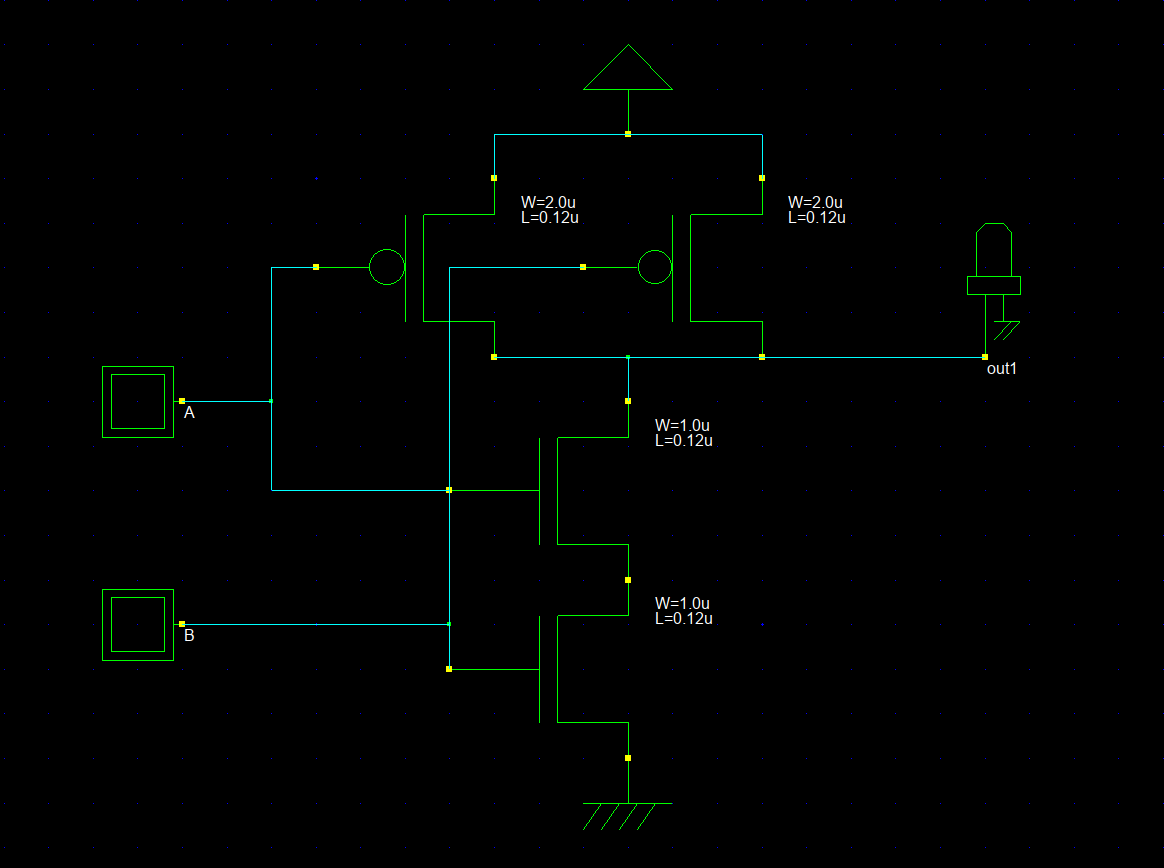
\includegraphics[width=0.8\textwidth]{2in-NAND.png}
    \caption{Schematic of the 2-input NAND}
\end{figure}

\subsection*{Observation}
From the simulation results in DSCH2, it was observed that the output of the 2-input NAND gate remains at logic HIGH for all input combinations except when both inputs A and B are logic HIGH. When either input is logic LOW, the output stays HIGH. The output transitions to logic LOW only for the input condition A = 1 and B = 1. These observations are fully consistent with the theoretical truth table of a 2-input NAND gate, confirming correct logical operation of the designed schematic.




\subsection{3-input NAND}
A 3-input NAND gate outputs a logic LOW only when all three inputs are logic HIGH. For any other input combination, the output remains logic HIGH.

\subsection*{Truth Table}
\begin{center}
\begin{tabular}{|c|c|c|c|}
\hline
A & B & C & Y \\ \hline
0 & 0 & 0 & 1 \\
0 & 0 & 1 & 1 \\
0 & 1 & 0 & 1 \\
0 & 1 & 1 & 1 \\
1 & 0 & 0 & 1 \\
1 & 0 & 1 & 1 \\
1 & 1 & 0 & 1 \\
1 & 1 & 1 & 0 \\ \hline
\end{tabular}
\end{center}

\subsection*{Schematic Image}
\begin{figure}[h!]
    \centering
    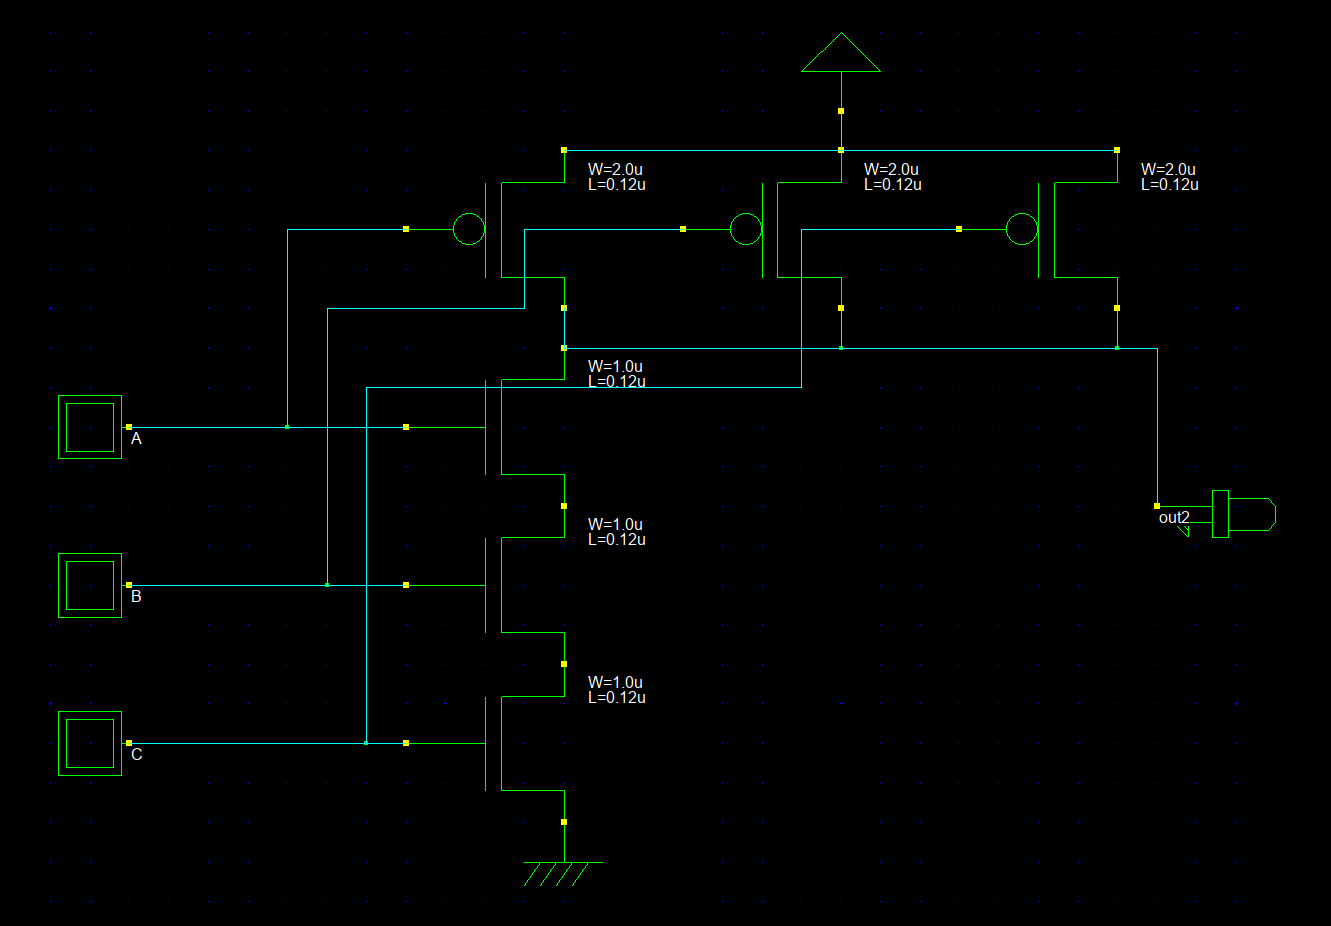
\includegraphics[width=0.7\textwidth]{3in-NAND.png}
    \caption{Schematic of the 3-input NAND}
\end{figure}

\subsection*{Observation}
From the truth table and simulation results, it was observed that the output of the 3-input NAND gate remains at logic HIGH for all input combinations except when all three inputs (A, B, and C) are simultaneously at logic HIGH. In the case where A = 1, B = 1, and C = 1, the output transitions to logic LOW. This behavior confirms that the gate performs the logical negation of the AND operation for three inputs. The observed output values from the DSCH2 simulation precisely matched the theoretical truth table, indicating correct functionality of the 3-input NAND gate.


% ---------------------------------------------------


\subsection{2-input NOR}
A 2-input NOR gate produces a logic HIGH output only when both inputs are logic LOW. For all other input combinations, the output is logic LOW. NOR gates are also universal gates in digital logic design.

\subsection*{Truth Table}
\begin{center}
\begin{tabular}{|c|c|c|}
\hline
A & B & Y \\ \hline
0 & 0 & 1 \\
0 & 1 & 0 \\
1 & 0 & 0 \\
1 & 1 & 0 \\ \hline
\end{tabular}
\end{center}

\subsection*{Schematic Image}
\begin{figure}[h!]
    \centering
    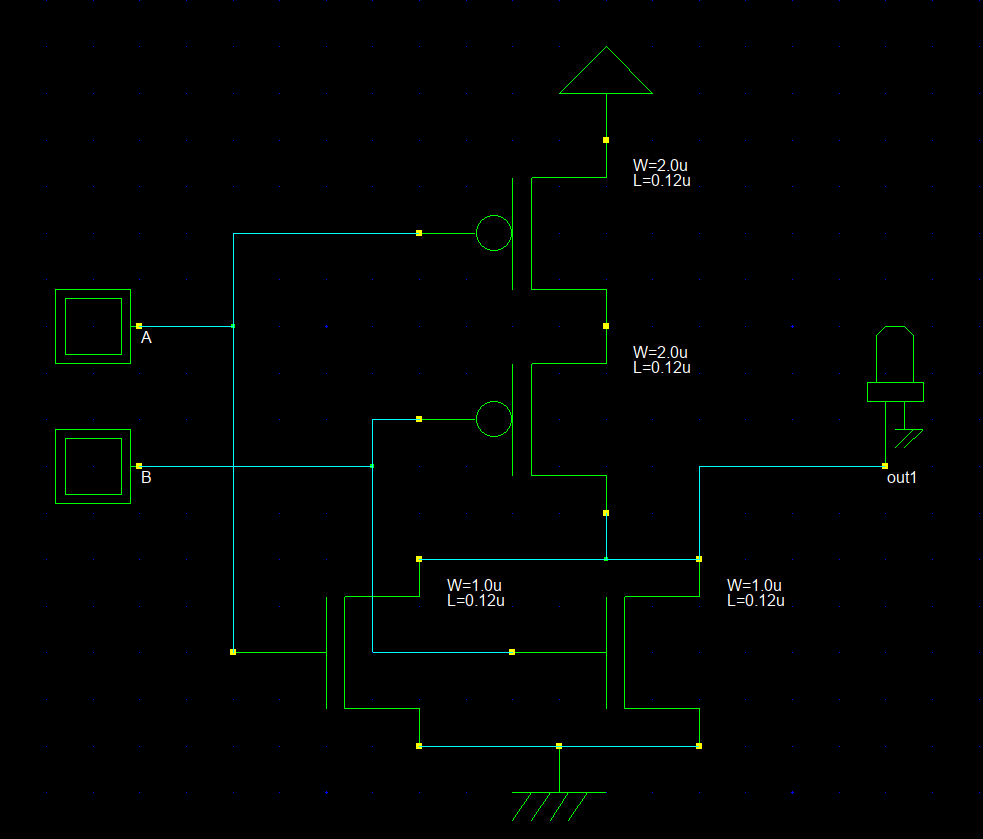
\includegraphics[width=0.8\textwidth]{2in-NOR.png}
    \caption{Schematic of the 2-input NOR}
\end{figure}


\subsection*{Observation}
From the truth table and simulation results, it is observed that the output of the 2-input NOR gate remains at logic HIGH only when both inputs A and B are at logic LOW. For all other input combinations where at least one input is logic HIGH, the output transitions to logic LOW. This behavior confirms that the circuit performs the logical NOR operation correctly, as verified through DSCH2 simulation.


% ---------------------------------------------------


\subsection{3-input NOR}

\subsection*{Truth Table}
\begin{center}
\begin{tabular}{|c|c|c|c|}
\hline
A & B & C & Y \\ \hline
0 & 0 & 0 & 1 \\
0 & 0 & 1 & 0 \\
0 & 1 & 0 & 0 \\
0 & 1 & 1 & 0 \\
1 & 0 & 0 & 0 \\
1 & 0 & 1 & 0 \\
1 & 1 & 0 & 0 \\
1 & 1 & 1 & 0 \\ \hline
\end{tabular}
\end{center}

\subsection*{Schematic Image}
\begin{figure}[h!]
    \centering
    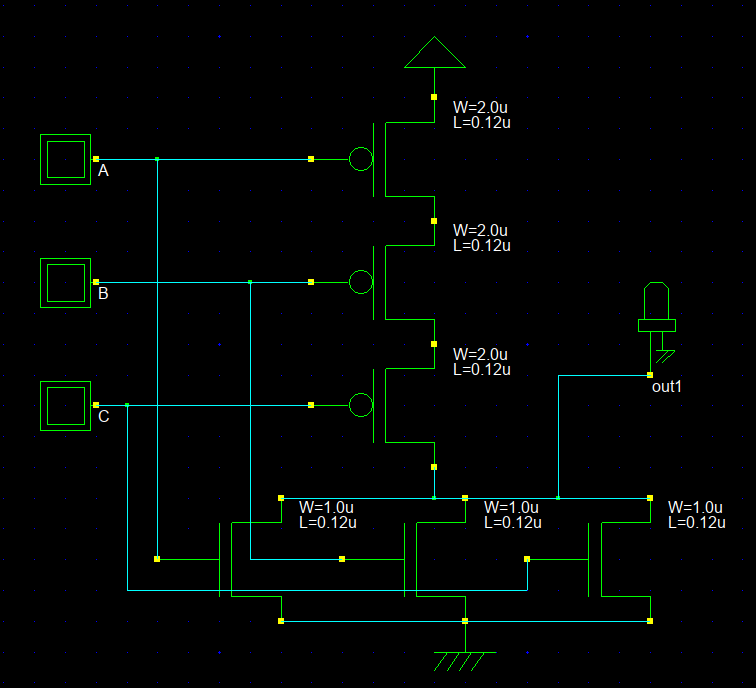
\includegraphics[width=0.65\textwidth]{3in-NOR.png}
    \caption{Schematic of the 3-input NOR}
\end{figure}

\subsection*{Observation}
From the simulation results, it is observed that the output of the 3-input NOR gate becomes logic HIGH only when all three inputs (A, B, and C) are at logic LOW. For any input combination where at least one input is HIGH, the output remains logic LOW. This behavior is consistent with the truth table of the 3-input NOR gate. The DSCH2 simulation output accurately reflects the expected NOR operation, confirming the correctness of the schematic design.


% ---------------------------------------------------


\subsection{AND Gate}
An AND gate outputs logic HIGH only when all inputs are HIGH.

\subsection*{Truth Table}
\begin{center}
\begin{tabular}{|c|c|c|}
\hline
A & B & Y \\ \hline
0 & 0 & 0 \\
0 & 1 & 0 \\
1 & 0 & 0 \\
1 & 1 & 1 \\ \hline
\end{tabular}
\end{center}

\subsection*{Schematic Image}
\begin{figure}[h!]
    \centering
    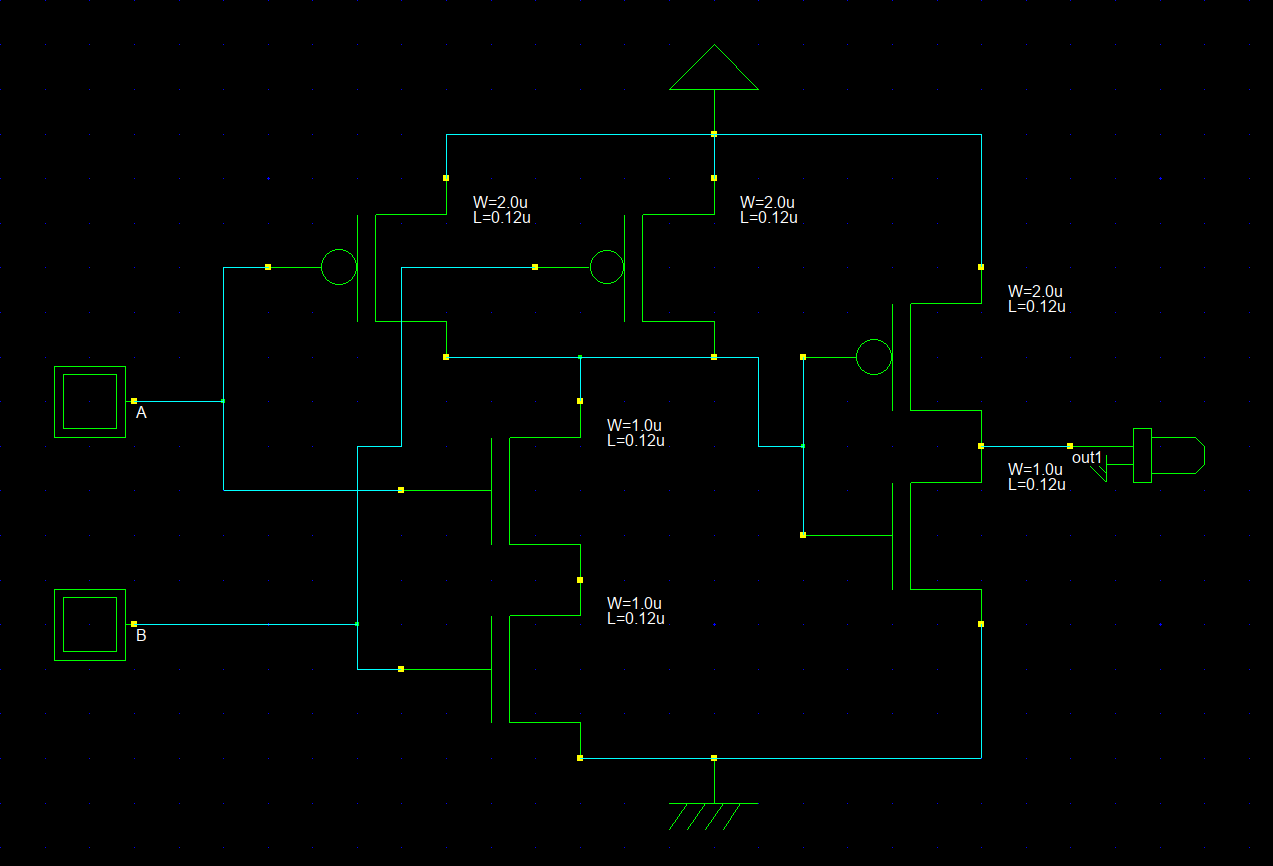
\includegraphics[width=1\textwidth]{2in-AND.png}
    \caption{Schematic of the AND Gate}
\end{figure}

\subsection*{Observation}
From the simulation results of the 2-input AND gate in DSCH2, it was observed that the output remains at logic LOW when any one or both of the inputs are at logic LOW. The output transitions to logic HIGH only when both inputs A and B are simultaneously at logic HIGH. This behavior is consistent with the truth table of an AND gate, confirming that the implemented schematic operates correctly.


% ---------------------------------------------------

\newpage
\subsection{OR Gate}
An OR gate produces logic HIGH when at least one input is HIGH.

\subsection*{Truth Table}
\begin{center}
\begin{tabular}{|c|c|c|}
\hline
A & B & Y \\ \hline
0 & 0 & 0 \\
0 & 1 & 1 \\
1 & 0 & 1 \\
1 & 1 & 1 \\ \hline
\end{tabular}
\end{center}

\subsection*{Schematic Image}
\begin{figure}[h!]
    \centering
    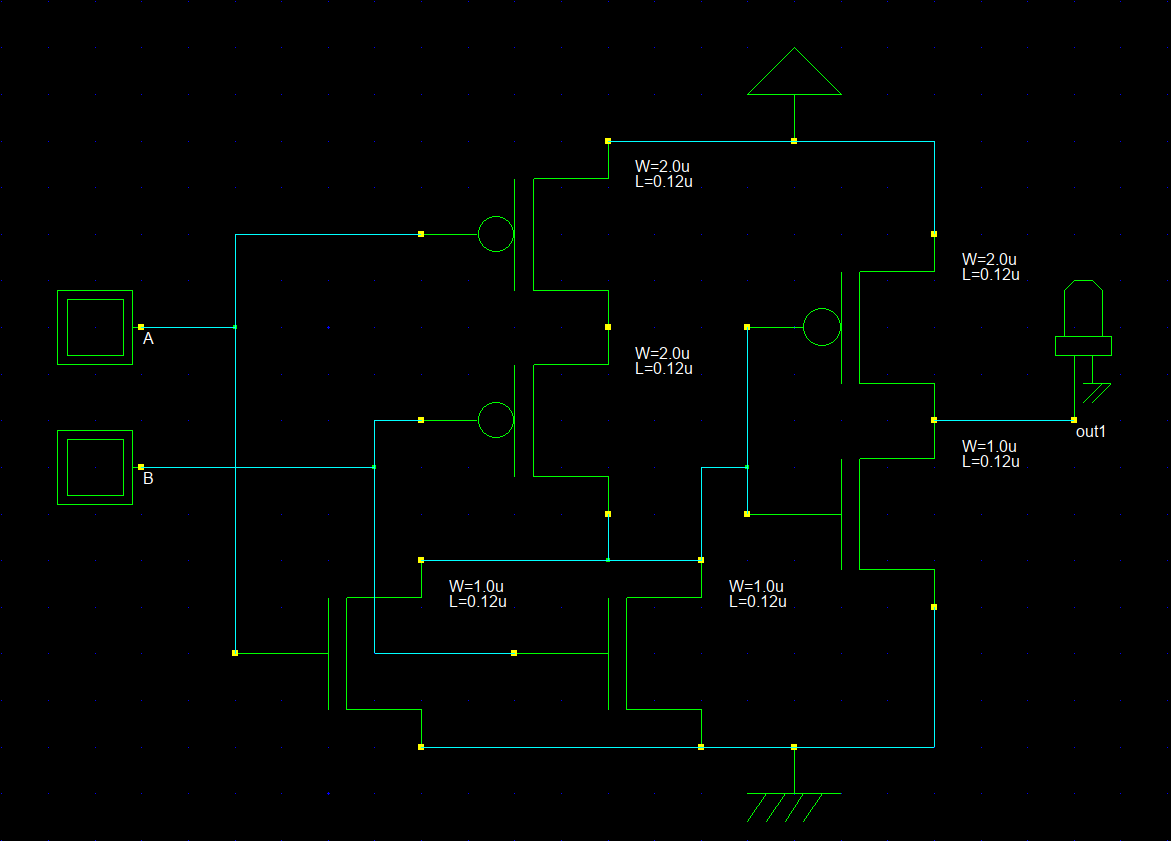
\includegraphics[width=1\textwidth]{2in-OR.png}
    \caption{Schematic of the OR Gate}
\end{figure}

\subsection*{Observation}
From the simulation results obtained in DSCH2, it was observed that the output of the 2-input OR gate becomes logic HIGH whenever at least one of the inputs is at logic HIGH. When both inputs A and B are at logic LOW, the output remains logic LOW. The simulation output exactly follows the theoretical truth table of the OR gate, confirming that the gate correctly performs the logical OR operation.



% ---------------------------------------------------


\subsection{XOR Gate}
An XOR gate outputs logic HIGH when the inputs are different.

\subsection*{Truth Table}
\begin{center}
\begin{tabular}{|c|c|c|}
\hline
A & B & Y \\ \hline
0 & 0 & 0 \\
0 & 1 & 1 \\
1 & 0 & 1 \\
1 & 1 & 0 \\ \hline
\end{tabular}
\end{center}

\subsection*{Schematic Image}
\begin{figure}[h!]
    \centering
    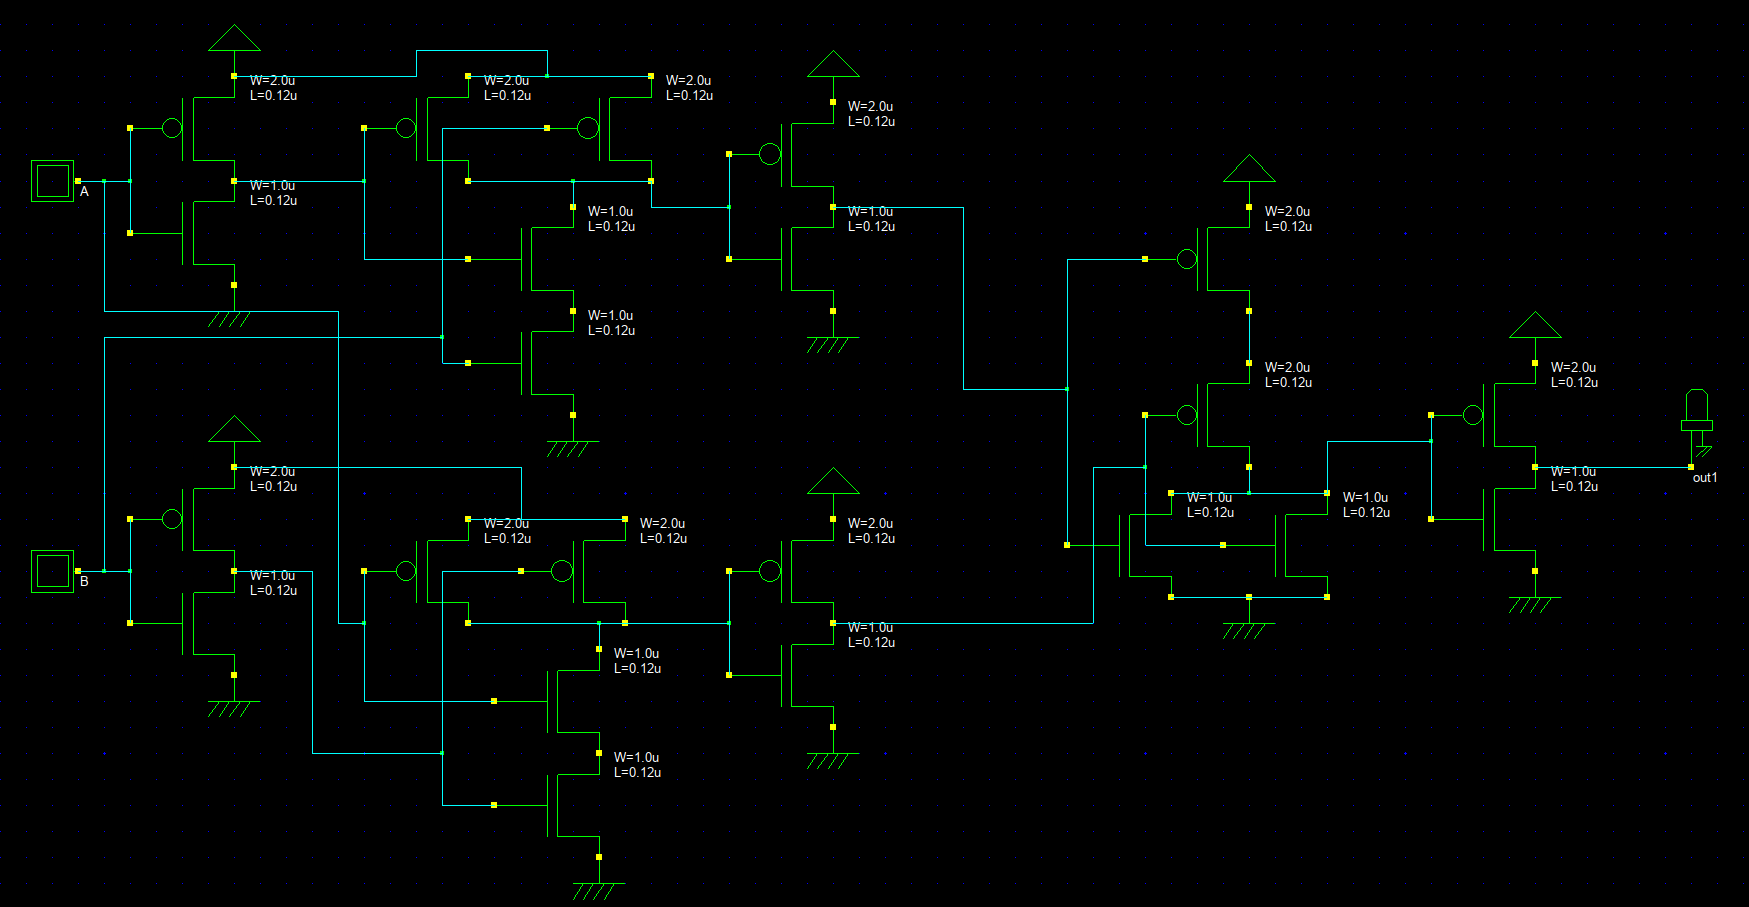
\includegraphics[width=1\textwidth]{2in-XOR.png}
    \caption{Schematic of the XOR Gate}
\end{figure}

\subsection*{Observation}
From the simulation results of the 2-input XOR gate in DSCH2, it was observed that the output remains logic LOW when both inputs are at the same logic level, i.e., when both inputs are LOW (0,0) or both inputs are HIGH (1,1). The output becomes logic HIGH when the inputs are different, i.e., for input combinations (0,1) and (1,0). These observations exactly match the theoretical truth table of the XOR gate, confirming that the circuit correctly performs the exclusive-OR operation.



\section{Conclusion}
In this laboratory exercise, schematic implementations of fundamental logic gates were created and simulated using the DSCH2 environment. For each gate, the simulated outputs matched the theoretical expectations based on Boolean logic. This laboratory reinforced the fundamental concepts of digital logic design and the practical use of DSCH2 for schematic entry and simulation.

\end{document}